\documentclass[a4paper, 11pt, oneside]{article}

\usepackage[utf8]{inputenc}
\usepackage[T1]{fontenc}
\usepackage[french]{babel}
\usepackage{array}
\usepackage{shortvrb}
\usepackage{listings}
\usepackage[fleqn]{amsmath}
\usepackage{amsfonts}
\usepackage{fullpage}
\usepackage{enumerate}
\usepackage{graphicx}             % import, scale, and rotate graphics
\usepackage{subfigure}            % group figures
\usepackage{alltt}
\usepackage{url}
\usepackage{indentfirst}
\usepackage{eurosym}
\usepackage{listings}
\usepackage{color}
\usepackage[table,xcdraw,dvipsnames]{xcolor}

% Change le nom par défaut des listing
\renewcommand{\lstlistingname}{Extrait de Code}

% Change la police des titres pour convenir à votre seul lecteur
\usepackage{sectsty}
\allsectionsfont{\sffamily\mdseries\upshape}
% Idem pour la table des matière.
\usepackage[nottoc,notlof,notlot]{tocbibind}
\usepackage[titles,subfigure]{tocloft}
\renewcommand{\cftsecfont}{\rmfamily\mdseries\upshape}
\renewcommand{\cftsecpagefont}{\rmfamily\mdseries\upshape}

\definecolor{mygray}{rgb}{0.5,0.5,0.5}
\newcommand{\coms}[1]{\textcolor{MidnightBlue}{#1}}

\lstset{
    language=C, % Utilisation du langage C
    commentstyle={\color{MidnightBlue}}, % Couleur des commentaires
    frame=single, % Entoure le code d'un joli cadre
    rulecolor=\color{black}, % Couleur de la ligne qui forme le cadre
    stringstyle=\color{RawSienna}, % Couleur des chaines de caractères
    numbers=left, % Ajoute une numérotation des lignes à gauche
    numbersep=5pt, % Distance entre les numérots de lignes et le code
    numberstyle=\tiny\color{mygray}, % Couleur des numéros de lignes
    basicstyle=\tt\footnotesize,
    tabsize=3, % Largeur des tabulations par défaut
    keywordstyle=\tt\bf\footnotesize\color{Sepia}, % Style des mots-clés
    extendedchars=true,
    captionpos=b, % sets the caption-position to bottom
    texcl=true, % Commentaires sur une ligne interprétés en Latex
    showstringspaces=false, % Ne montre pas les espace dans les chaines de caractères
    escapeinside={(>}{<)}, % Permet de mettre du latex entre des <( et )>.
    inputencoding=utf8,
    literate=
  {á}{{\'a}}1 {é}{{\'e}}1 {í}{{\'i}}1 {ó}{{\'o}}1 {ú}{{\'u}}1
  {Á}{{\'A}}1 {É}{{\'E}}1 {Í}{{\'I}}1 {Ó}{{\'O}}1 {Ú}{{\'U}}1
  {à}{{\`a}}1 {è}{{\`e}}1 {ì}{{\`i}}1 {ò}{{\`o}}1 {ù}{{\`u}}1
  {À}{{\`A}}1 {È}{{\`E}}1 {Ì}{{\`I}}1 {Ò}{{\`O}}1 {Ù}{{\`U}}1
  {ä}{{\"a}}1 {ë}{{\"e}}1 {ï}{{\"i}}1 {ö}{{\"o}}1 {ü}{{\"u}}1
  {Ä}{{\"A}}1 {Ë}{{\"E}}1 {Ï}{{\"I}}1 {Ö}{{\"O}}1 {Ü}{{\"U}}1
  {â}{{\^a}}1 {ê}{{\^e}}1 {î}{{\^i}}1 {ô}{{\^o}}1 {û}{{\^u}}1
  {Â}{{\^A}}1 {Ê}{{\^E}}1 {Î}{{\^I}}1 {Ô}{{\^O}}1 {Û}{{\^U}}1
  {œ}{{\oe}}1 {Œ}{{\OE}}1 {æ}{{\ae}}1 {Æ}{{\AE}}1 {ß}{{\ss}}1
  {ű}{{\H{u}}}1 {Ű}{{\H{U}}}1 {ő}{{\H{o}}}1 {Ő}{{\H{O}}}1
  {ç}{{\c c}}1 {Ç}{{\c C}}1 {ø}{{\o}}1 {å}{{\r a}}1 {Å}{{\r A}}1
  {€}{{\euro}}1 {£}{{\pounds}}1 {«}{{\guillemotleft}}1
  {»}{{\guillemotright}}1 {ñ}{{\~n}}1 {Ñ}{{\~N}}1 {¿}{{?`}}1
}
\newcommand{\tablemat}{~}

%%%%%%%%%%%%%%%%% TITRE %%%%%%%%%%%%%%%%
% Complétez et décommentez les définitions de macros suivantes :
\newcommand{\intitule}{Compléments de Programmation

Récursivité et Élimination de la Récursivité}
\newcommand{\Prenom}{Luca}
\newcommand{\Nom}{Matagne}
\newcommand{\matricule}{s190632}
% Décommentez ceci si vous voulez une table des matières :
\renewcommand{\tablemat}{\tableofcontents}

%%%%%%%% ZONE PROTÉGÉE : MODIFIEZ UNE DES DIX PROCHAINES %%%%%%%%
%%%%%%%%            LIGNES POUR PERDRE 2 PTS.            %%%%%%%%
\title{INFO0947: \intitule}
\author{\textsc{\Prenom}~\textsc{\Nom}, \matricule}
\date{}

\begin{document}
\maketitle
\newpage
\tablemat
\newpage
%%%%%%%%%%%%%%%%%%%% FIN DE LA ZONE PROTÉGÉE %%%%%%%%%%%%%%%%%%%%

%%%%%%%%%%%%%%%% RAPPORT %%%%%%%%%%%%%%%
% Complétez les sections ci-dessous

\section{Formulation Récursive}\label{formulation}
%%%%%%%%%%%%%%%%%%%%%%%%%%%%%%%%
\subsection{Définition récursive}
Nous observons que :

\begin{lstlisting}

Un nombre décimal est un nombre hexadécimal ayant subi une transformation et 
qu un nombre hexadécimal est un caractère représentant une puissance de 16
ajouté à la suite d une chaine de caractère représentant les puissance de 16
supérieures

\end{lstlisting}

Nous avons donc défini la structure « chaine de caractères(représentant un nombre
hexadécimal) »  récursivement. Nous allons donc formuler la transformation d’une
chaine de caractères en noombre décimaux sur base de cette définition récursive.

Appelons notre notation \textit{Traitement(s,n)}, avec \textit{s} une chaine de
caractères et \textit{n} sa longueur et appelons \textit{Transfo(s[n])} la 
transformation (permettant de passer de hexadécimal à décimal) de l'élément de 
rang n dans la chaine de caractères s.

\subsection{Cas de base}

Une chaine de caractères composée d'un seul caractère est une chaine de caractère
représentant la puissance 0 de 16 en nombre hexadécimal.
Lorsq'uon lui applique la transformation en nombre décimal, on obtient le résultat suivant: 

\centerline{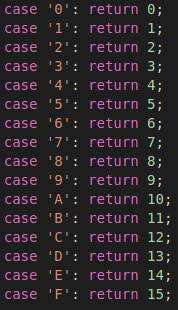
\includegraphics[height=8cm, width=3cm]{AA.png}}

Exemple:

\begin{center}
s={'A,/0'}

\textit{\textbf{Traitement(s,1)=Transfo(s[0])=11}}
\end{center}

\subsection{Cas récursif}

Pour déterminer le cas récursif, observons un exemple:

\begin{center}
\textbf{'A23' $\rightarrow$ 2595}
\end{center}

Imaginons que l$'$on découpe la chaine \textbf{'A23'} selon la définition 
récursive, on a

\begin{center}
\textbf{'A2 || 3' $\rightarrow$ 'A2' + 3 $*$ 1}    

$=$

\textbf{'A2 || 3' $\rightarrow$ 'A2' + 3}

(Le 3 après le $+$ est bien le nombre décimal et plus le caractère)
\end{center}

Et puis,

\begin{center}
\textbf{'A || 23' $\rightarrow$ 'A' + 2$*$16 + 3$*$1}

$=$

\textbf{'A || 23' $\rightarrow$ 'A' + 35}
\end{center}

On voit qu'il faut stocker le résultat du traitement du caractère et l'additioner
au résultat du traitement sur une chaine examptée du caractère que l'on vient de
traiter.

\begin{center}
\textit{\textbf{Traitement(s, n) = Traitement(s[n], n) + Traitement(s, n-1)}}
\end{center}

\subsection{Synthèse}



\section{Spécification}\label{specification}
%%%%%%%%%%%%%%%%%%%%%%%%%
%
% Fournissez et discutez ici la spécification formelle de la fonction
% hexa_dec_rec()
%

\section{Construction Récursive}\label{recur}
%%%%%%%%%%%%%%%%%%%%%%%%%%%%%%%%%
%
% Fournissez et discutez ici la construction formelle (avec les assertions
% intermédiaires) de la fonction hexa_dec_rec()
%

\section{Traces d'Exécution}\label{traces}
%%%%%%%%%%%%%%%%%%%%%%%%%%%%%
%
% Fournissez et discutez ici les traces d'exécution de la fonction romain_rec()
% pour les exemples donnés dans l'énoncé
%

% L'exemple ci-dessous donne une trace d'exécution pour un exercice sur les
% Piles (cfr. GameCodes associés).  Inspirez-vous du code LaTeX pour produire
% vos traces d'exécution.
% \begin{tabular}{|c|}
% \\
% \\
% \textcolor{white}{--}\\
% \hline
% \end{tabular}~~
% \begin{tabular}{|c|}
% \\
% \\
% 20\\
% \hline
% \end{tabular}~~
% \begin{tabular}{|c|}
% \\
% 4\\
% 20\\
% \hline
% \end{tabular}~~
% \begin{tabular}{|c|}
% \\
% \\
% 80\\
% \hline
% \end{tabular}~~
% \begin{tabular}{|c|}
% \\
% 9\\
% 80\\
% \hline
% \end{tabular}~~
% \begin{tabular}{|c|}
% 7\\
% 9\\
% 80\\
% \hline
% \end{tabular}~~
% \begin{tabular}{|c|}
% \\
% 16\\
% 80\\
% \hline
% \end{tabular}~~
% \begin{tabular}{|c|}
% \\
% \\
% 5\\
% \hline
% \end{tabular}

\section{Complexité}\label{complexite}
%%%%%%%%%%%%%%%%%%%%%
%
% Fournissez et discutez ici la complexité théorique de la fonction
%  hexa_dec_rec()
%

\section{Dérécursification}\label{derecur}
%%%%%%%%%%%%%%%%%%%%%%%%%%%%
%
% Fournissez et discutez ici la dérécursification de la fonction hexa_dec_rec()
% Attention, il n'est pas question ici de fournir un algorithme itératif mais
% bien d'éliminer la récursivité comme cela a été vu au cours.
% La solution doit être proposée en utilisant le pseudo-code vu au cours (et
% dans les GameCodes du Chapitre 9).
%

\end{document}
